\chapter{Konzeption des Schlussfolgerer}

TEXT

\section{MEMA-Prinzip}
\label{abschnitt-mema-prinzip}
Die Idee des MEMA-Prinzips stammt aus der Diplomarbeit von Timo Weithöhner \cite{Weithoehner}. Es ermöglicht die Abspeicherung einer Ontologie in eine Datenbank mit einem festen Satz von Tabellen. Dies vereinfacht es Regeln in SQL zu erstellen, da diese vorformuliert werden können.

Diese Diplomarbeit hat aufgezeigt, das die Umwandlung und Abspeicherung einer Ontologie in einen fixen Satz von Relationen möglich ist, so dass danach eine effiziente Schlussfolgerung durchgeführt werden kann.

Das ursprüngliche MEMA-Prinzip von Timo Weithöhner ist um folgende Punkte erweitert.
Es wurde erstmal auf den erweiterten Sprachschatz von OWL2 RL angepasst. Was aber besonders zu erwähnen ist sind die Relationen \emph{list} und \emph{history} \ref{relations-list-history}. Sie speichern keine Axiome wie alle anderen. Die Relation list dient als Hilfstruktur für Axiome, die eine variable Anzahl von Elementen abspeichern. Die Relation history wird benutzt, um den Abhängigkeitsverlauf beim inferieren von Fakten speichern zu können. Damit ist es möglich Ableitungen gezielt wieder rückgängig zu machen. Deswegen sind auch alle anderen Relationen mit einer \emph{id} Spalte ausgestattet, die Axiome bzw. komplexe Unterausdrücke eindeutig identifiziert.

Allgemein wurde bei der Erstellung der Tabellenstruktur darauf geachtet, das die Formulierung der Regeln in SQL vereinfacht wird. So ist im Normalfall die Ergebnismenge einer Regel dadurch zu erhalten, in dem man die beteiligten Relationen miteinander joinet auf den Variablen, die in den Regeln angegeben sind.

Die Gattung der relational database management systems wird shcon seit den 1970er Jahren entwickelt. Sie entstammen nicht nur dem theoretischen Gebiet, sondern freuen sich vor allem in der Praxis großer Beliebtheit. Durch die einheitliche Abfragesprache SQL sind fast alle heutigen Systeme anzusprechen. Dadurch konnte sich eine Vielzahl von Systemen auf dem Markt etablieren. Durch diese Auswahl kann man sich aussuchen, welches System am  besten zu den gewünschten Anforderung passt und bei Änderungen der Anforderungen kann das System leicht durch ein anderes ausgetauscht werden. Durch den hohen Einsatz in der PRaxis haben sich äußerst robuste, schnelle und skalierbare Lösungen entwickelt. Durch den Einsatz einens RDBMS bekommt man folgendes Wissen, Erfahrung und Vorteile ``gratis'':
\begin{itemize}
  \item Schnelle und geprüfte Algorithmen
  \item Robustheit, durch die \emph{ACID}-Eigenschaft auch im parallelisierten Betrieb
  \item Caching
  \item Modularität
  \item geringere Codegröße
\end{itemize}

In den Diagrammen sind Spalten, die ``fett'' markiert sind mit einem Index ausgestattet. Felder die Unterstrichend sind wurden in der Datenbank als Primärschluss umgesetzt und müssen eindeutig in der Relation sein.

\tikzstyle{relation}=[rectangle, draw=black, rounded corners, fill=white, drop shadow, text justified, anchor=north, text=black, text width=4cm]

\begin{figure}
	\caption{Die Hilfsrelationen list und history}
	\label{relations-list-history}
\begin{center}
	\begin{tikzpicture}[node distance=6cm]
		\node (history) [relation, rectangle split, rectangle split parts=2]{
				\textbf{history}
			\nodepart{second}
				\underline{id}: INT\newline
				\underline{table}: TABLE\newline
				\underline{sourceId}: INT\newline
				\underline{sourceTable}: TABLE
		};
		\node (list) [relation, rectangle split, rectangle split parts=2, left of= history]{
				\textbf{list}
			\nodepart{second}
				id: INT\newline
				\textbf{\underline{name}}: CLASS\newline
				\textbf{\underline{element}}: CLASS/IND
		};
	
	\end{tikzpicture}
\end{center}
\end{figure}

\tikzstyle{relation}=[rectangle, draw=black, rounded corners, fill=white, drop shadow, text justified, anchor=north, text=black, text width=5cm]
\begin{figure}
	\caption{Liste der Relationen, für die auch Fakten erzeugt werden}
	\label{relations-for-which-data-is-created}
\begin{center}
	\begin{tikzpicture}[node distance=2.5cm]
		\node (subClass) [relation, rectangle split, rectangle split parts=2]{
				\textbf{subClass}
			\nodepart{second}
				\underline{id}: INT\newline
				\textbf{\underline{sub}}: CLASS\newline
				\textbf{\underline{super}}: CLASS
		};
		
		\node (equivalentClass) [relation, rectangle split, rectangle split parts=2, right =2cm of subClass]{
				\textbf{equivalentClass}
			\nodepart{second}
				\underline{id}: INT\newline
				\textbf{\underline{left}}: CLASS\newline
				\textbf{\underline{right}}: CLASS
		};
		
		\node (subProperty) [relation, rectangle split, rectangle split parts=2, below of= subClass]{
				\textbf{subProperty}
			\nodepart{second}
				\underline{id}: INT\newline
				\textbf{\underline{sub}}: PROPERTY\newline
				\textbf{\underline{super}}: PROPERTY
		};
		
		\node (equivalentProperty) [relation, rectangle split, rectangle split parts=2, right =2cm of subProperty]{
				\textbf{equivalentProperty}
			\nodepart{second}
				\underline{id}: INT\newline
				\textbf{\underline{left}}: CLASS\newline
				\textbf{\underline{right}}: CLASS
		};
		
		
		\node (classAssertionEnt) [relation, rectangle split, rectangle split parts=2, below of= subProperty]{
				\textbf{classAssertionEnt}
			\nodepart{second}
				\underline{id}: INT\newline
				\textbf{\underline{entity}}: IND/CLASS\newline
				\textbf{\underline{class}}: CLASS
		};
		
		\node (classAssertionLit) [relation, rectangle split, rectangle split parts=2, right =2cm of classAssertionEnt]{
				\textbf{classAssertionLit}
			\nodepart{second}
				\underline{id}: INT\newline
				\textbf{\underline{literal}}: LITERAL\newline
				\textbf{\underline{class}}: CLASS\newline
				\textbf{\underline{language}}: LANGUAGE
		};
		
		\node (sameAsEnt) [relation, rectangle split, rectangle split parts=2, below =1.5cm of classAssertionEnt]{
				\textbf{sameAsEnt}
			\nodepart{second}
				\underline{id}: INT\newline
				\textbf{\underline{left}}: IND\newline
				\textbf{\underline{right}}: IND
		};
		
		\node (sameAsLit) [relation, rectangle split, rectangle split parts=2, right =2cm of sameAsEnt, text width=6cm]{
				\textbf{sameAsLit}
			\nodepart{second}
				\underline{id}: INT\newline
				\textbf{\underline{left}}: IND\newline
				\textbf{\underline{right}}: IND\newline
				\textbf{\underline{left\_type}}: CLASS\newline
				\textbf{\underline{right\_type}}: CLASS\newline
				\textbf{\underline{left\_language}}: LANGUAGE\newline
				\textbf{\underline{right\_language}}: LANGUAGE
		};
		
		\node (objectPropertyAssertion) [relation, rectangle split, rectangle split parts=2, below =1.8cm of sameAsEnt]{
				\textbf{objectPropertyAssertion}
			\nodepart{second}
				\underline{id}: INT\newline
				\textbf{\underline{subject}}: IND\newline
				\textbf{\underline{property}}: PROPERTY\newline
				\textbf{\underline{object}}: IND
		};
		
		\node (dataPropertyAssertion) [relation, rectangle split, rectangle split parts=2, right =2cm of objectPropertyAssertion, text width=6cm]{
				\textbf{dataPropertyAssertion}
			\nodepart{second}
				\underline{id}: INT\newline
				\textbf{\underline{subject}}: IND\newline
				\textbf{\underline{property}}: PROPERTY\newline
				\textbf{\underline{object}}: LITERAL\newline
				\textbf{\underline{type}}: CLASS\newline
				\textbf{\underline{language}}: LANGUAGE
		};
		
		 
		\node (propertyDomain) [relation, rectangle split, rectangle split parts=2, below= 1cm of objectPropertyAssertion]{
				\textbf{propertyDomain}
			\nodepart{second}
				\underline{id}: INT\newline
				\textbf{\underline{property}}: CLASS\newline
				\textbf{\underline{domain}}: CLASS
		};
		
		\node (propertyRange) [relation, rectangle split, rectangle split parts=2, right =2cm of propertyDomain]{
				\textbf{propertyRange}
			\nodepart{second}
				\underline{id}: INT\newline
				\textbf{\underline{property}}: CLASS\newline
				\textbf{\underline{range}}: CLASS
		};
	
	\end{tikzpicture}
\end{center}
\end{figure}

Die Abbildung \ref{relations-for-which-data-is-created} sind Relationen für die neue Fakten abgeleitet werden können. Alle anderen Relationen werden nur beim laden einer Ontologie gefüllt und danach nicht mehr verändert.

\begin{figure}
	\caption{Relationen die auf Listen arbeiten}
	\label{relations-that-work-on-lists}
\begin{center}
	\begin{tikzpicture}[node distance=3cm]
		\node (members) [relation, rectangle split, rectangle split parts=2]{
				\textbf{members}
			\nodepart{second}
				id: INT\newline
				\textbf{\underline{class}}: CLASS\newline
				\textbf{\underline{list}}: NAME
		};
		
		\node (propertyChain) [relation, rectangle split, rectangle split parts=2, right =2cm of members]{
				\textbf{propertyChain}
			\nodepart{second}
				id: INT\newline
				\textbf{\underline{property}}: PROPERTY\newline
				\textbf{\underline{list}}: NAME
		};
		
		\node (hasKey) [relation, rectangle split, rectangle split parts=2, below of= members]{
				\textbf{hasKey}
			\nodepart{second}
				id: INT\newline
				\textbf{\underline{class}}: CLASS\newline
				\textbf{\underline{list}}: NAME
		};
		
		\node (intersectionOf) [relation, rectangle split, rectangle split parts=2, right =2cm of hasKey]{
				\textbf{intersectionOf}
			\nodepart{second}
				id: INT\newline
				\textbf{\underline{class}}: CLASS\newline
				\textbf{\underline{list}}: NAME
		};
		
		\node (unionOf) [relation, rectangle split, rectangle split parts=2, below of= hasKey]{
				\textbf{unionOf}
			\nodepart{second}
				id: INT\newline
				\textbf{\underline{class}}: CLASS\newline
				\textbf{\underline{list}}: NAME
		};
		
		
		\node (oneOf) [relation, rectangle split, rectangle split parts=2, right= 2cm of unionOf]{
				\textbf{oneOf}
			\nodepart{second}
				id: INT\newline
				\textbf{\underline{class}}: CLASS\newline
				\textbf{\underline{list}}: NAME
		};
	
	\end{tikzpicture}
\end{center}
\end{figure}
Die Relationen aus Abbildung \ref{relations-that-work-on-lists} sind alle Relationen die mit einer variablen Anzahl von Elementen umgehen und daher mit Listen arbeiten. Es gibt Relationen wie sameAs und differentFrom die mehrere Fakten enthalten können. Hier ist es so festgelegt, das wenn nur ein Paar erzeugt wird, dann wird es in der speziellen Relation abgelegt. Falls die Anzahl größer ist wird es in der members Relation abgelegt. Hier gilt aber ebenfalls das neue Fakten nur für Relationen in der Abbildung \ref{relations-for-which-data-is-created} erzeugt werden können, d.h. es können nur paarweise Daten erzeugt werden und keine Liste.\footnote{Die Bennenung der Spalten ist vereinfacht gegenüber der Umsetzung in der Datenbank, das es hier reservierte Schlüselwörter gibt. Außerdem sind Spalten nicht wirklich von dem angegeben Typ. Es soll damit aufgezeigt werden, das sehr wohl klar ist in welcher Tabelle welche Fakten abgespeichert werden. Auch wenn die Grenzen zwischen A-Box und T-Box verschwimmen, werden sie trotzdem nicht durcheinander gebracht.}

\tikzstyle{relation}=[rectangle, draw=black, rounded corners, fill=white, drop shadow, text justified, anchor=north, text=black, text width=6cm]
\begin{figure}
	\caption{sonstige Relationen}
	\label{relations-others-1}
\begin{center}
	\begin{tikzpicture}[node distance=2.7cm]
		\node (allValuesFrom) [relation, rectangle split, rectangle split parts=2]{
				\textbf{allValuesFrom}
			\nodepart{second}
				id: INT\newline
				\textbf{\underline{part}}: CLASS\newline
				\textbf{\underline{property}}: CLASS\newline
				\textbf{\underline{total}}: NAME
		};
		
		\node (someValuesFrom) [relation, rectangle split, rectangle split parts=2, right =1cm of allValuesFrom]{
				\textbf{someValuesFrom}
			\nodepart{second}
				id: INT\newline
				\textbf{\underline{part}}: CLASS\newline
				\textbf{\underline{property}}: CLASS\newline
				\textbf{\underline{total}}: NAME
		};
		
		\node (hasValueEnt) [relation, rectangle split, rectangle split parts=2, below =0.7cm of allValuesFrom]{
				\textbf{hasValueEnt}
			\nodepart{second}
				id: INT\newline
				\textbf{\underline{class}}: CLASS\newline
				\textbf{\underline{property}}: PROPERTY\newline
				\textbf{\underline{value}}: IND
		};
		
		\node (hasValueLit) [relation, rectangle split, rectangle split parts=2, right =1cm of hasValueEnt]{
				\textbf{hasValueLit}
			\nodepart{second}
				id: INT\newline
				\textbf{\underline{class}}: CLASS\newline
				\textbf{\underline{property}}: PROPERTY\newline
				\textbf{\underline{value}}: LITERAL\newline
				\textbf{\underline{language}}: LANGUAGE\newline
				\textbf{\underline{type}}: CLASS
		};
		
		\node (disjointWith) [relation, rectangle split, rectangle split parts=2, below =0.7cm of hasValueEnt]{
				\textbf{disjointWith}
			\nodepart{second}
				id: INT\newline
				\textbf{\underline{left}}: CLASS\newline
				\textbf{\underline{right}}: CLASS
		};
		
		\node (propertyDisjointWith) [relation, rectangle split, rectangle split parts=2, right =1cm of disjointWith]{
				\textbf{propertyDisjointWith}
			\nodepart{second}
				id: INT\newline
				\textbf{\underline{left}}: PROPERTY\newline
				\textbf{\underline{right}}: PROPERTY
		};
		
		\node (maxCardinality) [relation, rectangle split, rectangle split parts=2, below of= disjointWith]{
				\textbf{maxCardinality}
			\nodepart{second}
				id: INT\newline
				\textbf{\underline{class}}: CLASS\newline
				\textbf{\underline{property}}: PROPERTY\newline
				\textbf{\underline{value}}: NUMBER
		};
		
		\node (maxQualifiedCardinality) [relation, rectangle split, rectangle split parts=2, right =1cm of maxCardinality]{
				\textbf{maxQualifiedCardinality}
			\nodepart{second}
				id: INT\newline
				\textbf{\underline{class}}: CLASS\newline
				\textbf{\underline{property}}: PROPERTY\newline
				\textbf{\underline{total}}: CLASS\newline
				\textbf{\underline{value}}: NUMBER
		};
		
		\node (complementOf) [relation, rectangle split, rectangle split parts=2, below of= maxCardinality]{
				\textbf{complementOf}
			\nodepart{second}
				id: INT\newline
				\textbf{\underline{left}}: CLASS\newline
				\textbf{\underline{right}}: CLASS
		};
		
		\node (inverseOf) [relation, rectangle split, rectangle split parts=2, right =1cm of complementOf]{
				\textbf{inverseOf}
			\nodepart{second}
				id: INT\newline
				\textbf{\underline{left}}: CLASS\newline
				\textbf{\underline{right}}: CLASS
		};
		
		\node (negativeObjectPropertyAssertion) [relation, rectangle split, rectangle split parts=2, below of= complementOf]{
				\textbf{negativeObjectPropertyAssertion}
			\nodepart{second}
				id: INT\newline
				\textbf{\underline{subject}}: IND\newline
				\textbf{\underline{property}}: PROPERTY\newline
				\textbf{\underline{object}}: IND
		};
		
		\node (negativeDataPropertyAssertion) [relation, rectangle split, rectangle split parts=2, right =1cm of negativeObjectPropertyAssertion]{
				\textbf{negativeDataPropertyAssertion}
			\nodepart{second}
				id: INT\newline
				\textbf{\underline{subject}}: IND\newline
				\textbf{\underline{property}}: PROPERTY\newline
				\textbf{\underline{object}}: IND
		};
		
		\node (differentFromEnt) [relation, rectangle split, rectangle split parts=2, below = 1cm of negativeObjectPropertyAssertion]{
				\textbf{differentFromEnt}
			\nodepart{second}
				id: INT\newline
				\textbf{\underline{left}}: IND\newline
				\textbf{\underline{right}}: IND
		};
		\node (differentFromLit) [relation, rectangle split, rectangle split parts=2, right =1cm of differentFromEnt]{
				\textbf{differentFromLit}
			\nodepart{second}
				id: INT\newline
				\textbf{\underline{left}}: IND\newline
				\textbf{\underline{right}}: IND\newline
				left\_language: LANGUAGE\newline
				left\_type: CLASS\newline
				right\_language: LANGUAGE\newline
				right\_type: CLASS
		};
		
	\end{tikzpicture}
\end{center}
\end{figure}

Die sonstige Relationen aus Abbildung \ref{relations-others-1} sind so umfangreich, da in OWL2 RL fast die komplette Sprachmächtigkeit von OWL2 abbildbar ist.


\section{Optimierungen für das MEMA-Prinzip}

Im Paper Classifying $\mathcal{ELH}$ Ontologies in SQL Databases \cite{Delaitre2009} sind interessante Ansätze für Verbesserungen.

Zum einen wird eine Normalisierung vorgeschlagen. Diese ist über zwei Wege möglich:
\begin{itemize}
  \item Vereinheitlichung von strukturell gleichen Ausdrücken. Das bedeutet, das wenn die selben Ausdrücke mehrmals in einer Ontologie vorkommen, z.B. als Teile in einem komplexeren Ausdruck, werden alle diese gleichen Unterausdrücke nur einmal abgespeichert. Das hat den Vorteil, dass es den Speicherplatz verringert und über den selben Ausdruck nicht mehrmals geschloßen wird. Dies ist mit der OWLAPI sogar relativ leicht möglich, da sie schon von selbst strukturelle gleiche Ausdrücke zusammenfasst. Allerdings wurde diese Optimierung nicht umgesetzt, den für die Möglichkeit abgeleitete Fakten wieder zu löschen muss der Weg wie Fakten entstanden sind eindeutig sein. Hier würde man aber Probleme verursachen. Diese Optimierung ist grundsätzlich nicht ausgeschloßen. Für den Fall, dass man nichts löschen müsste könnte sie direkt umgesetzt werden. Für den Fall das man etwas löschen will, müsste man etwas geschickter Vorgehen. Auf diese Optimierung wurde auf Grund ihrer Komplexität in diesem Fall verzichtet.
  \item Umwandlung gewisser Konstrukte. Es wird außerdem vorgeschlagen manche Konstrukte umzuwandeln, so z.B. $A \sqsubseteq B \land C \Rightarrow A \sqsubseteq B, A \sqsubseteq C$. Damit könnte man sich manche Regeln sparen. Inwieferen dies im RL Fragment nützlich ist, da hier doch recht viele Konstrukte aus OWL2 zu gelassen sind und welche Regeln man damit wirklich einsparen kann ist eine offene Frage.
\end{itemize}


Desweitern wird beschrieben, wie sie die Leistung beim Laden der Ontologie steigern. Hier werden ebenfalls zwei Tricks verwendet:
\begin{itemize}
  \item Zum einen wird die Ontologie \emph{on-the-fly} in die Datenbank geschrieben, d.h. während die Ontologie gelesen wird wird sie auch parallel in die Datenbank geschrieben. Das hat den Vorteil das sie nicht zweimal durchlaufen werden muss. Die OWLAPI lässt zwar auch die Serialisierung direkt in eine Datenbank zu. Das Laden der Ontologie in die OWLAPI und den Schlussfolgerer ist aus den folgenden Gründen entkoppelt. Zum einen kann es sein, dass man die OWLAPI ersteinmal läd und erst später den Schlussfolgerer dazu startet. So ist zumindest der normale Ablauf. Hier würde ein solche Optimierung also nichts bringen. Zweitens müsste man sich bei einer direkten Serialisierung um alle Konstrukte in einer Ontologie kümmern und nicht nur um die, die man zum ableiten verwendet. Es würde also den Schlussfolgerer komplexer in seinem Aufbau machen.
  \item Es werden Konstrukte immer in eine \emph{in-memory} Relation eingefügt und dann in größeren Blöcken auf einmal rausgeschrieben. Ob diese Optimierung wirklich soviel bringt ist fraglich, da ein gutes Datenbanksystem ein solches Caching von alleine betreiben sollte. Außerdem liegt der Overhead dabei vermutlich eher beim parsen der vielen INSERT Statements. Trotzdem könnte man diese Optimierung in betracht ziehen. Sie wurde ebenfalls aus Komplexitätsgrunden außer Acht gelassen.
\end{itemize}

\subsection{Andere Serialisierungsmöglichkeiten}
Die OWLAPI bietet eine Reihe von Formaten zur Serialisierung von OWL-Ontologien an. Diese sind zum Teil auch in der Spezifikation von OWL erwähnt. Das Problem was allen Formatne gemein ist, ist das es einfach Textformate sind die entweder vollständig in den Hauptspeicher eingelsen werden müssen oder nur sehr langsame Zugriffsmöglihckeiten anbieten.

Dieses Problem wurde schon von mehreren erkannt \cite{Kleb2009ProtegeDB}, \cite{Kleb2009OWLDB} und versucht durch eine Abbildung in einer Datenbank zu lösen.

Hier ist das Problem einerseits, dass sich diese Paper noch mit der OWLAPIv3 beschäftigen nud andererseits ist es ja nicht das Ziel dieser Diplomarbeit  eine Serialisierungsmöglichkeit für eine komplete Ontologie in einer Datenbank zu finden, sondern nur die nötigen Fakten abzulegen, um darauf gut Regeln in SQL abbilden zu können.

\section{Wissensrepräsentation in Zusammenhang mit einem Schlussfolgerer}

Die Formalismus einer Wissensrepräsentation hängt nicht direkt mit dem Kalkül zusammen, wenn man allerdings über die gewünschte Wissensrepräsentation bescheid weiß, ist es möglich den Schlussfolger daraufhin zu optimieren. Im Falle dieser Arbeit wird mit einer Wissensrepräsentation gearbeitet -- OWL2 RL -- und der Schlussfolgerer ist daraufhin optimiert, die in der Sprache repräsentierten Kriterien, wie Entscheidbarkeit und Komplexität zu erreichen.

Das bedeutet zum einen, das wenn die Sprache entscheidbar ist, also es einen terminierenden Alogrithmus gibt. Das ist durch zwei Dinge zu erreichen, ein gutes Design, welches diesen Algorithmus überhaupt ermöglicht und eine fehlerfreie Programmierung. Diese beiden Dinge sind natürlich nie so in der Praxis zu ereichen, aber es wurde versucht den Code und die Architektur so einfach und verständlich wie möglich zu halten, um Fehler schnell zu finden.

Die Komplexität einer Sprache gibt nur eine obere Schranke, den sog. \emph{worst-case} an, der für eine Lösungsfindung nötig ist. Die Umsetzung in einem Programm muss diesen dann erst noch erreichen. Das wird im hier behandelten Schlussfolgerer versucht zu erreichen, indem man sich nur auf eine Wissensrepräsentation konzentriert. Damit können die Regeln zur Wissensgewinnung nahe an der Definition der Sprache umgesetzt werden und somit auch nicht schlechter als die theoretischen Komplexität wird.
Die anderen Kriterien spielen für den Schlussfolgerer nur eine untergeordnete Rolle.

\section{Aufbau des Schlussfolgerers}


\begin{figure}[htp]
	\caption{Aufbau der Hauptklassen des U2R3 Reasoner}
	\label{schema-aufbau-u2r3}
	
	\tikzstyle{composition}=[->, >=diamond, thick]
	
	\tikzstyle{class}=[rectangle, draw=black, rounded corners, fill=white, drop shadow, text centered, anchor=north, text width=3.5cm, rectangle split, rectangle split parts=1]

	\begin{tikzpicture}[node distance=2cm]
	    \node (U2R3Reasoner) [class]
	        {
	            \textbf{U2R3Reasoner}
	%            \nodepart{second}name
	        };
	        
	    \node (RuleManager) [class, below of= U2R3Reasoner]
	        {
	            \textbf{RuleManager}
	%            \nodepart{second}name
	        };
	        
	     \node (RelationManager) [class, left =0.1cm of RuleManager]
	        {
	            \textbf{RelationManager}
	%            \nodepart{second}name
	        };
	        
	    \node (ReasonProcessor) [class, right =0.1cm of RuleManager]
	        {
	            \textbf{ReasonProcessor}
	            %\nodepart{second}+ classify()
			};

		\draw[composition] (RuleManager.north) -- (U2R3Reasoner.south);
		\draw[composition] (RelationManager.north) -- (U2R3Reasoner.south);
		\draw[composition] (ReasonProcessor.north) -- (U2R3Reasoner.south);

	\end{tikzpicture}
\end{figure}

Das Klassendiagram in Abbildung \ref{schema-aufbau-u2r3} stellt den vereinfachten Aufbau des Schlussfolgerers dar. Die Aufgaben des Reasoner sind dabei in vier Hauptbereich zerlegt.
\begin{enumerate}
  \item Der RelationManger verwaltet die Relationen in der Datenbank und stellt die Verbindung zu dieser her. Darin sind alle Methoden die mit der Erstellung und Veränderung von Tabellenstrukturen zu tun hat enthalten.
  \item Der RuleManager kapselt alle Regeln ab.
  \item Der ReasonProcessor bringt Regeln zur Ausführung. Damit ist er das eigentliche Herz des Schlussfolgerers. Hier wird bestimmt welche Regeln auf welche Relationen angewendet werden und in welcher Reihenfolge.
  \item Der U2R3Reasoner stellt die Schnittstelle nach außen dar. Er nimmt Ontologien, sowie Anfragen an diese Ontologien entgegen.
\end{enumerate}

\section{Arbeitsablauf des Schlussfolgerers}

In der nachfolgenden Abbildung \ref{image-u2r3-workflow} ist der gewöhnliche Ablauf des Reasoner dargestellt. Dabei ist er in drei Phasen einzuteilen. Das Laden der Ontologie, der Schlussfolgerungsvorgang und die Abfrage.

\begin{figure}
	\caption{Arbeitsablauf des Schlussfolgerers}
	\label{image-u2r3-workflow}
\begin{center}
	\scalebox{0.6}{
		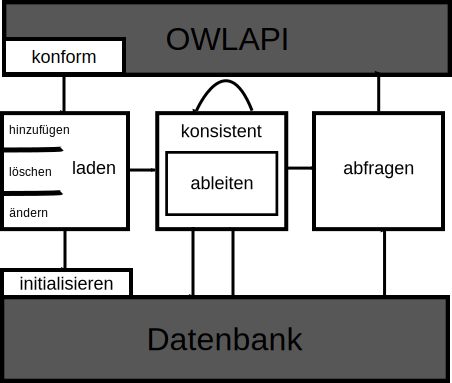
\includegraphics{images/u2r3-workflow.pdf}
	}
\end{center}
\end{figure}

\subsection{Konformität}
Konformität: überprüft, ob die verwendete Syntax im OWL2 RL Profil liegt
laden: bringt die Ontolgoie in das Datenbank-Schema, dabei merkt es an welche Regeln für das ableiten ausgeführt werden sollen
initialisieren: erzeugt das Datenbankschema notfalls, läd Standardwerte und richtet in der Datenbank nötige Funktionen ein
konsistent: ist eine Hülle um dafür zu sorgen, das nur über konsistente Fakten geschlossen wird. Die Häufigkeit kann eingestellt werden.
ableiten:Wendet die Ableitungsregeln an. Die Regelandwendung ist abgschloßen wenn keine neuen Fakten erzeugt werden können.
abfragen: implementiert die Schnittstelle der OWLAPI, mit der man Anfragen an die abgeleiteten Fakten stellen kann

\subsection{OWLAPI Anbindung}

Der obere Teil ist die sogenannte OWLAPI. Die OWLAPI ist eine Bibliothek die das Auslesen von Ontologien in verschiedenen Formaten erlaubt und eine Schlussfolgererschnittstelle für andere Programme zur Verfügung stellt. Durch die Implementierung dieser Schnittstelle in U2R3 ist es für alle Programme zugänglich die mit der OWLAPI arbeiten.
Die Schnittstelle stellt dabei auch eine Liste typischer Abfragen für einen Reasoner dar und kann allein dadurch schon als Messlatte für die Fähigkeiten eines Schlussfolgerers verwendet werden. Das OWLAPI-Projekt ist open-source und in Java implementiert und ist damit auch optimal für die Implementierung von U2R3 geeignet. Neben der reinen Parsertätigkeit kann die OWLAPI auch noch helfen zu überprüfen, ob eine Ontologie im OWL2 RL Profil liegt und nimmt damit weitere Arbeit ab.

\subsection{Das Laden einer Ontologie}

Die Inhalte einer Ontolgie die für das Schlussfolgern wichtig sind, sind die Axiome. Axiome sind dabei Fakten die als allgemein gültig angenommen werden. Sie dienen dazu das Universum der Ontologie zu modellieren und einen Startpunkt für weitere Schlussfolgerungen zu erzeugen.

Alle Axiome werden entsprechend dem MEMA-Prinzip abgelegt. Dabei ist für jedes Axiom genau eine Relation vorgesehen. Falls die Ontologie nicht OWL2 RL konform ist müssen für gewisse Axiome implizite Informationen abgelegt, wie. z.B.

\begin{table}
	\caption{Eine implizite Regel}
	\label{rule-impl}
\begin{center}
	\begin{tabular}{l|l}
    If & then \\ \hline
	T(?i1, ?property, ?i2 ) & T(?property owl:type ObjectProperty) \\
   \end{tabular}
\end{center}
\end{table}


Falls ein Axiom aus komplexen Ausdrücken zusammengesetzt ist werden die Ausdrücke rekursiv abgearbeitet und einzeln behandelt. Zum herstellen der Beziehungen bei komplexen Axiomen werden Platzhalter für die Ausdrücke verwendet. Die Platzhalter die dabei erzeugt werden stammen von der OWLAPI aus der NodeID Klasse und folgen damit dem selben Schema wie auch bei anonymen Individuen.

In folgendem Besipeil soll der komplexe Ausdruck $A \sqcap \exists p.B \sqsubseteq C$ abgespeichert werden. Zur Verdeutlichung wurden Klammern eingebaut.

\begin{equation}
\overbrace{
	(\overbrace{A \sqcap (
		\overbrace{\exists{}p.B}
		^{nid3 \Rightarrow someValuesFrom(nid3, p, B)})}
	^{nid2 \Rightarrow intersectionOf(nid1, nid2), list(nid2, A, nid3)})}
^{nid1 \Rightarrow subClass(nid1, C)} \sqsubseteq C
\end{equation}
Wenn ein Ausdruck nicht direkt abgespeichert werden kann,, dann wird für den Unterausdruck eine \emph{NodeID} erzeugt. Im obigen Beispiel werden drei Stück davon erzeugt. Diese stehen stellvertretend für den Unterausdruck. Es wird dann rekursiv weitergearbeitet bis alle in einfache Ausdrücke aufgelöst werden konnte.

Wenn Fakten in eine Relation geschrieben werden, wird von dieser ein Hinweis (\emph{Reason}) an den Regelprozessor geschickt.

Dieser überprüft die Ursache und legt entsprechende Regeln an, die auf diese Veränderung ausgeführt werden können.

Die abzuarbeitenden Regeln enthalten eine Referenz auf die Fakten, die hinzugekommen sind. Allgemein sind sie so implementiert, das sie nur auf diesen neuen Fakten arbeiten -  auf den sogenannten Deltas - dies ist allerdings nicht in allen Fällen möglich (\emph{cls-int1}), sinnvoll (zu viele verschiedene Kombinationsmöglichkeiten) oder einfach zu komplex und damit fehleranfällig (\emph{prp-spo2}). Falls zwei oder mehrmals eine Regel auf die selben neuen Fakten erzeugt wird bevor sie ausgelöst wird, werden die beiden Regeln zu einer zusammengefasst und können je nach Einstellung neu priorisiert werden.

All diese Regeln sind in einer Warteschleife abgelegt, die beim Laden der Ontologie gefüllt wird und beim Abarbeiten, d.h. dem Realisieren, der Ontologie ausgelesen wird.

Regeln können durch das Erzeugen von neuen Fakten Hinweise für den Regelprozessor geben der daraufhin weitere Regeln anlegt und in die Warteschlange einsortiert.

Der Vorgang des Realisierens ist abgeschlossen, wenn keine Regel neue Fakten und damit neue Regeln erzeugen kann.

Der OWL2 RL Regelsatz garantiert dabei, das es immer zu einem Ende der Regelanwendung kommen wird, egal ob eine gültige oder ungültige Ontologie geladen wird.

Für das Abarbeiten und Erzeugen der Regeln ist hauptsächlich der Regelprozessor verantwortlich. Hier sind noch weitere Einstellungsmöglichkeiten, wie z.B. die parallele Verarbeitung von Regeln vorhanden.


\subsection{Das Schlussfolgern in einer Ontologie}
Das Schlussfolgern in einer Ontologie besteht darus die möglichen Regeln der OWL2 RL SPzeifiaktion anzuwenden. Diese Regeln erzeugen neue Fakten oder überpürfen dieKonsistenz. Der Schlussfolgerer hat seine Arbeit erledigt, wenn keine Regel neue Fakten erzeugen kann, Das sicherzustellen und dabei möglichst wenige Regeln anzuwenden ist seine Aufgabe. Daher wird im folgenden äher beschrieben, wann welche Regeln ausgelöst werden und in welcher Rehenfolge sie angewendet werden.

\subsubsection{Auswertungsstrategien}
Die Auswertungstrategie beschreibt in welcher Reihenfolge der Regelprozessor die Anwendung von Regeln auslöst. 

Der naive Ansatz wäre alle Regeln nacheinander auszuführen, d.h. alles Regeln die implementiert sind anwenden, wenn eine der Regeln dabei neue Fakten erzeugt muss dieser Vorgang wiederholt werden. Dieses Vorgehen ist trotz seiner leichten Umsetzbarkeit nicht implementiert, da der Reasoner damit unnötig viel Arbeit verrichten müssste.

Ein etwas fortgeschrittener Ansatz ist es die Abhängigkeiten der Regeln auszunutzen, d.h. nur wenn für die Prämisse einer Regel überhaupt Fakten vorhanden sind kann diese ausgelöst werden. Das heißt im konkreten, wenn eine Relation die in einer Regel in der Prämisse verwendet wird neue Daten enthält, dann muss diese Regel ausgelöst werden. Dieses Verfahren ist im Schlussfolgerer so umgesetzt.

Es wurde allerdings diese Vorgehen noch etwas weiter verbessert. Veränderungen in verschiedenen Tabellen könnten mehrmals die selbe Regel auslösen, da die Regel mehrere Vorbedingungen  hat. Die Regel wird dann nicht mehrfach ausgelöst sondern es werden erst alle Regeln in eine Warteschlange gesammelt. Wird eine neue Regel ausgelöst wird dann zuerst geschaut, ob diese Regel schon in der Warteschlange vorhanden ist.

Außerdem gibt es hier noch eine Optimierungsmöglichkeit, mit der man noch experimentieren kann. Wenn eine Regel in der Warteschlange erneut eingereiht werden soll, kann man sich entscheiden, ob die Regel an ihrere Stelle in der Schlange verbleibt oder ob sie herausgenommen wird und wieder ans Ende gestellt. Welches der beiden Verfahren besser ist muss sich erst noch in der Praxis zeigen.

In der Konfiguration des u2r3 ist diese Einstellungsmöglichkeit unter dem Namen \emph{EvaluationStrategy} zu finden. Gültige Werte dafür sind \emph{COMMONLAST} oder \emph{RARELAST}

\subsubsection{Regelauslösung}
Für jede Manipulation der Datenbank (DELETE/INSERT) wird eine Reason ausgelöst. Es wird dabei nur eine Reason ausgelöst, egal wieviele Zeilen von der Manipulation betroffen waren. Eine Reason löst dann weitere Actions aus, je nachdem welche Regeln davon betroffen sind.

\begin{verbatim}
DB Manipulation (1) ===> (1) Reason (1) ===> (n) RuleActions
\end{verbatim}


\begin{verbatim}
           Realtion                     Delta
            ######
            ######         <===           #
            ######
                                          |
(welche Regel) |                          | (welche neuen Daten)
               |                          |
                ####>  Reason  <==========

                          | (1)
                          |
                          | (eine Regel mit neuen Daten)
                          |
                          v (n)

                      RuleAction
\end{verbatim}


\subsection{Das Abfragen einer Ontologie}
Das Abfragen in einer Ontologie lässt sich grundlegend in zwei Arten aufteilen. Erstens man hat einen Ausdruck und möchte überpürfen, ob dieser geschlussfolgert worden ist. Diese Art von Abfrage liefert nur ja oder nein zurück. Die zweite Art von Abfrage möchte eine Ergebnismenge zurück. Dabei ist im Gegensatz zur ersten Art von Abfrage eine Variable in der Abfrage, die gefüllt wird.

Bei beiden ist grundsätzlich so, dass das ``Anfrage'' OWL-Konstrukt in eine SQL-ABfrage umgeformt wird. In beiden Fällen kann die Abfrage beantwortet werden egal on die SQL-ABfrage etwas zurückbringt oder nicht. Im zweiten Fall muss aber bei einem Ergebnis daraus noch eine Ergebnis ereugt werden, so das es dem OWLAPI Format entspricht.

\section{Komplexe Ausdrücke}
Was sind komplexe Ausdrücke?
\subsection{Komplexe Ausdrücke finden}
Einfügen von Statements oder Werten nicht gut, weil darüber nicht geschloßen werden kann bzw. wenn darüber Aussagen gemacht werden sollen muss erst geschloßen werden. (zeitaufwendig!)


\section{Zurückziehen von Fakten}
Das Einfügen von Fakten, die man löschen will, um herauszufinden, welche gleich sind, um sie danach wieder zu löschen macht keinen großen Sinn. Erstens ist es Recht aufwendig zu implementieren. Zweitens müsste nach dem Einfügen neuer Fakten ersteinmal wieder die Ableitungsregeln ausgeführt werden. Das zerstört den Vorteil, den man sich durch forward-chaining mit direct-materialisation erkauft hat sofort wieder und bringt außerdem auch Nachteile mit sich wenn man noch nicht komplett fertig war mit dem Schlussfolgern.
Daher muss es ein Verfahren geben die zu löschenden Fakten zu finden ohne sie vorher einfügen zu müssen.
\begin{verbatim} 
* Wie können spätere Manipluationen durchgeführt werden?
* Was ist der Aufwand nach einer Änderung (von Fakten oder Konzepten)?
\end{verbatim}
